\newpage
\section{Cut Continuous Interior Penalty Method for the Biharmonic Problem}%
\label{sec:cutcip_biharmonic_problem}


Questions arise when we want to allow for complex geometries where some physical domain $\Omega $ has a smooth boundary $\Gamma $ and, thus, cannot be fully covered of a fitted mesh. This motivated us to define a unfitted finite element method.
The concept is to generate a structured background mesh which fully covers $\Omega $ , but does necessarily fit it perfectly. Conceptionally, is the bilinear form $a_{h}( \cdot ,\cdot ) $  and linear form $l_{h}( \cdot ) $  still associated with the
physical domain with the discrete space $V_{h}$ defined in the unfitted mesh. However, we will run into geometrical problems when
so-called cut finite elements has a very small intersection of the physical domain, i.e, $\abs{ T \cap \Omega  }_{d} \ll \abs{ T }_{d}  \lesssim h^{d}$ and $\abs{ \Gamma \cap T }_{d} \ll  h^{d-1}$, where $\abs{ \cdot  }_{d} $ is the
measure of the volume in dimension $d$.
The cut elements are identified as a crucial geometric issue since the inverse inequalities outlined in Subsection \ref{sub:some_general_inequalities} do not generalize well to these elements. This highlights challenges in establishing stability and a priori estimates for any geometric arrangement.

One way do handle this issue is to introduce the so-called cut finite element method (CutFEM).
The method is adding an stabilization term, also known as the so-called ghost penalty term, which extends the finite element space from the interior elements outside the physical domain  stable way which also guarantees stabilization and geometrical robustness.
optimal approximation properties. For more information, see
\cite{burman2015cutfem, burman2010ghost, burman2022cutfem, burman2012fictitious}.
Utilizing a corresponding CutFEM DG elliptic framework \cite{gurkan2019stabilized} and starting from the CIP methods introduced in Section \ref{sec:CIP_biharmonic_problem}, is the goal in this section to engineer a suitable stabilized ghost penalty
term for the biharmonic problem.
We will show what assumptions that is needed for the ghost-penalty method for the discrete problem to be stable in Subsection \ref{sub:stability_estimate} and obtain optimal convergence in Subsection \ref{sec:a_priori_estimates}.  Once
this is fulfilled will we propose a $g_{h}$ which fulfills these assumptions in Subsection \ref{sec:constructing_ghost_penalties}.


\subsection{Computational domain}%
\label{sub:unfitted_mesh}

\begin{figure}[h!]
    \centering
\subfloat[]{\label{a1}
        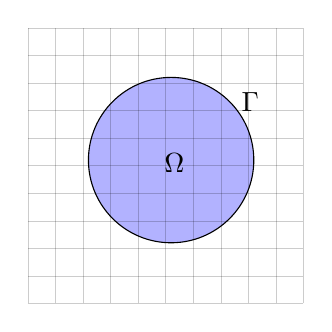
\begin{tikzpicture}[scale=0.7]

            \draw[fill=blue!30] (0.1, 0.1) circle (1.5cm);
            % Background mesh
            \foreach \i in {-2.5, -2, ..., 2.5} {
                \draw[line width=0.1pt, shift={(-2.5,\i)}, opacity=0.2] (0,0) -- (5,0);
                \draw[line width=0.1pt, shift={(\i,-2.5)}, opacity=0.2] (0,0) -- (0,5);
            }


            % Labels
            \node[below right] at (-0.2,0.4) {$\Omega$};
            \node[below right] at (1.2,1.5) {$\Gamma$};
        \end{tikzpicture}

}\hfill
\subfloat[]{\label{a}
        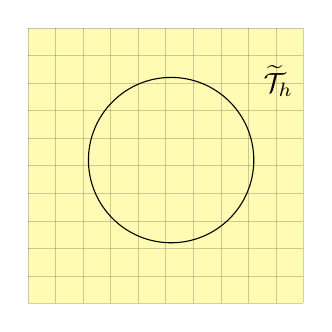
\begin{tikzpicture}[scale=0.7]

            \fill[yellow!30] (-2.5,2.5) -- (2.5,2.5) -- (2.5,-2.5) -- (-2.5,-2.5) -- cycle;

            \draw (0.1, 0.1) circle (1.5cm);
            % Background mesh
            \foreach \i in {-2.5, -2, ..., 2.5} {
                \draw[line width=0.1pt, shift={(-2.5,\i)}, opacity=0.2] (0,0) -- (5,0);
                \draw[line width=0.1pt, shift={(\i,-2.5)}, opacity=0.2] (0,0) -- (0,5);
            }


            % Labels
            \node[below right] at (1.6,2.0) {$\widetilde{\mathcal{T}}_{h}$};
        \end{tikzpicture}

}\hfill
\subfloat[]{\label{c}
        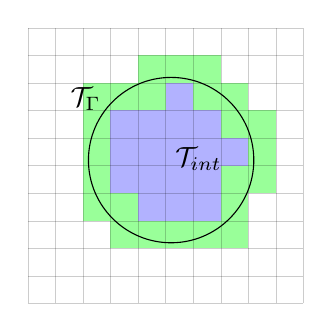
\begin{tikzpicture}[scale=0.7]

            % POTENTIAL ACTIVE MESH
            \fill[blue!30] (2,2) -- (2,-1.5) --(-1.5,-1.5) -- (-1.5,2) -- cycle;

            % ELEMENTS WITH NO INTERSECTION
            % lower left
            \fill[white] (-1.5,-1.5) rectangle (-1.0,-1.0);
            \fill[white] (-1.5,2.0) rectangle (-1.0,1.5);
            \fill[white] (-1.0,2.0) rectangle (-0.5,1.5);
            \fill[white] (2,2) rectangle (1.5,1.5);
            \fill[white] (1.5,2) rectangle (1.0,1.5);
            \fill[white] (2,1.5) rectangle (1.5,1.0);
            \fill[white] (1.5,-1) rectangle (2,-1.5);
            \fill[white] (1.5,-0.5) rectangle (2,-1.0);

            % CUT ELEMENTS
            \fill[green!40] (-0.5,2.0) rectangle (1.0,1.5);
            \fill[green!40] (-1.5,1.5) rectangle (0.0,1.0);
            \fill[green!40] (0.5,1.5) rectangle (1.5,1.0);
            \fill[green!40] (-1.5,1.0) rectangle (-1.0,-1.0);
            \fill[green!40] (-1.0,-0.5) rectangle (-0.5,-1.5);
            \fill[green!40] (-0.5,-1.5) rectangle (1.5,-1.0);
            \fill[green!40] (1.5,-1) rectangle (1.0,-0.0);
            \fill[green!40] (1.5,-0.5) rectangle (2.0,1.0);
            \fill[green!40] (1.0,0.5) rectangle (1.5,1.0);

            \draw (0.1, 0.1) circle (1.5cm);
            % Background mesh
            \foreach \i in {-2.5, -2, ..., 2.5} {
                \draw[line width=0.1pt, shift={(-2.5,\i)}, opacity=0.2] (0,0) -- (5,0);
                \draw[line width=0.1pt, shift={(\i,-2.5)}, opacity=0.2] (0,0) -- (0,5);
            }


            % Labels
            \node[below right] at (0.0,0.5) {$\mathcal{T}_{int}$};
            \node[below right] at (-1.9,1.6) {$\mathcal{T}_{\Gamma }$};
        \end{tikzpicture}
}
\hfill
\subfloat[]{\label{b}
        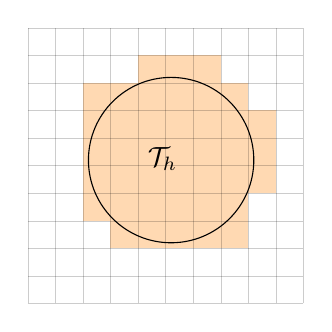
\begin{tikzpicture}[scale=0.7]

            % POTENTIAL ACTIVE MESH
            \fill[orange!30] (2,2) -- (2,-1.5) --(-1.5,-1.5) -- (-1.5,2) -- cycle;

            % ELEMENTS WITH NO INTERSECTION
            % lower left
            \fill[white] (-1.5,-1.5) rectangle (-1.0,-1.0);
            \fill[white] (-1.5,2.0) rectangle (-1.0,1.5);
            \fill[white] (-1.0,2.0) rectangle (-0.5,1.5);
            \fill[white] (2,2) rectangle (1.5,1.5);
            \fill[white] (1.5,2) rectangle (1.0,1.5);
            \fill[white] (2,1.5) rectangle (1.5,1.0);
            \fill[white] (1.5,-1) rectangle (2,-1.5);
            \fill[white] (1.5,-0.5) rectangle (2,-1.0);

            % CUT ELEMENTS
            \fill[orange!30] (-0.5,2.0) rectangle (1.0,1.5);
            \fill[orange!30] (-1.5,1.5) rectangle (0.0,1.0);
            \fill[orange!30] (0.5,1.5) rectangle (1.5,1.0);
            \fill[orange!30] (-1.5,1.0) rectangle (-1.0,-1.0);
            \fill[orange!30] (-1.0,-0.5) rectangle (-0.5,-1.5);
            \fill[orange!30] (-0.5,-1.5) rectangle (1.5,-1.0);
            \fill[orange!30] (1.5,-1) rectangle (1.0,-0.0);
            \fill[orange!30] (1.5,-0.5) rectangle (2.0,1.0);
            \fill[orange!30] (1.0,0.5) rectangle (1.5,1.0);

            \draw (0.1, 0.1) circle (1.5cm);
            % Background mesh
            \foreach \i in {-2.5, -2, ..., 2.5} {
                \draw[line width=0.1pt, shift={(-2.5,\i)}, opacity=0.2] (0,0) -- (5,0);
                \draw[line width=0.1pt, shift={(\i,-2.5)}, opacity=0.2] (0,0) -- (0,5);
            }


            % Labels
            % \node[below right] at (2.5,2.5) {$\widetilde{\mathcal{T}}_{h}$};
            % \node[below right] at (0.4,0.5) {$\mathcal{T}_{int}$};
            \node[below right] at (-0.5,0.5) {$\mathcal{T}_{h }$};
        \end{tikzpicture}


}


\caption{Illustration of the domain $\Omega$ with the corresponding boundary $\Gamma$, the background mesh $\widetilde{\mathcal{T}}_{h} $,  the cut cells $\mathcal{T} _{\Gamma }$, the interior cells $\mathcal{T} _{int}$ and the active set $\mathcal{T} _{h} =
\mathcal{T}_{ int } \cup \mathcal{T}_{ \Gamma  }  $. }
\label{fig:background_mesh}
\end{figure}


We want to devise a CutFEM based on the CIP formulation for the biharmonic problem. Assume that the physical domain $\Omega \subseteq    \mathbb{R} ^d$ to be open and bounded with a corresponding a sufficiently smooth boundary $\Gamma  $.
 Let $\widetilde{\mathcal{T}_{h} } $ be a shape-regular and quasi-uniform mesh which covers $\Omega $, but does not need to fit the
domain. Let us denote the active set $\mathcal{T} _{h} \subseteq \widetilde{\mathcal{T}_{h}}$ which intersects the interior of the active domain $\Omega $, that is
\begin{equation}
\label{eq:active_set}
\mathcal{T} _{h} = \left\{ T \in \widetilde{\mathcal{T} }_{h}  \mid  T \cap \Omega   \neq \emptyset    \right\}.
\end{equation}
We define the corresponding set of interior facets, \[
    \mathcal{F} _{h}^{int} = \left\{ F = T^{+} \cap T^{-}  \mid  T^{+}, T^{-} \in \mathcal{T} _{h} \text{ and } T^{+} \neq T^{-} \right\},
\]
and the set of elements cut by the boundary \[
\mathcal{T} _{\Gamma } = \left\{ T \in \mathcal{T} _{h}   \mid  T \cap \Gamma \neq \emptyset  \right\}.
\]
For convenience, will we define also the interior of the active set as $\mathcal{T} _{int}$.
\[
\mathcal{T} _{int} = \left\{ T \in \mathcal{T} _{h}   \mid  T \cap  \mathrm{Int}(\Omega ) \neq \emptyset  \right\}.
\]
Hence, we have that the active set is the union of the interior and cut elements, $\mathcal{T} _{h} = \mathcal{T} _{int} \cup  \mathcal{T} _{\Gamma }$. For an illustration, see Figure \ref{fig:background_mesh}.



\subsection{ Cut Continuous Interior Penalty Method }%
\label{sub:cut_cip_method}

% This makes it natural to redefine the biharmonic problem on a unfitted domain.
% Let $\Omega \subseteq    \mathbb{R} ^d$ s.t. $\Gamma  $ be its corresponding boundary in $C^2$. Then is the biharmonic problem on the form,
% \begin{subequations}
% \label{eq:bi_main_problem2}
% \begin{align}
%     \Delta^2  u  + \alpha  u  & = f( x)  \quad \text{in } \Omega,   \label{eq:bi_main_problem2_a}\\
%     \partial _{n} u & = g_{1}(x)   \quad \text{on } \Gamma ,  \label{eq:bi_main_problem2_b}\\
%     \partial _{n} \Delta  u & = g_{2}( x)   \quad \text{on } \Gamma .  \label{eq:bi_main_problem2_c}
% \end{align}
% \end{subequations}
% Here is $\Delta ^2 = \Delta  \left( \Delta  \right) $ the biharmonic operator, also known as the bilaplacian. We will assume for the strong form that $u \in H^{4}\left( \Omega  \right) $, $\alpha  >0 $ and $f \in L^{2}\left( \Omega  \right)
% $.

% For completeness will we also add the corresponding continuous weak formulation.
% Let $ V := \left\{ v \in H^2( \Omega )  \mid \partial _{n} v = g_{1} \right\}  $.
% \begin{equation}
% \label{eq:bi_weak_cut}
% \text{Find } u \in V   \text{ such that } a( u,v) = l( v)  \forall v \in V
% \end{equation}
% where
% \begin{equation}
%     \begin{split}
% a( u,v) & =  ( \alpha u,v)_{\Omega } + ( \Delta u, \Delta v)_{\Omega } - (  \Delta u, \partial _{n} v) _{\Gamma }\\
% l( v)  &= ( f,v)_{\Omega } - ( g_{2} , v)_\Omega
%     \end{split}
% \end{equation}

% \begin{remark}
%     Be aware that the only difference between the strong BH variants, \eqref{eq:bi_problem} and \eqref{eq:bi_main_problem2}, is that the first one problem is fitted s.t. $\mathcal{T}_{h} = \Omega  $, while the latter is unfitted and equipped with a
%     sufficiently smooth boundary. The continuous weak formulations and \eqref{eq:cont_weak_problem} and \eqref{eq:bi_weak_cut} is entirely identical in its composition.
% \end{remark}




% \begin{enumerate}[label=\arabic*)]
%     \item Assume $g_{1}( x) = 0 $. Then unfitted Hessian formulation has the bilinear form

% \begin{equation}
%         \label{eq:cip_unfitted_hessian_form}
% \begin{split}
% a_{h}^{H} \left( u, v \right)   =&   \left( \alpha  u, v \right) _{\mathcal{T} _{h} \cap \Omega }   +  \left( D^2 u, D^2v \right) _{\mathcal{T} _{h} \cap \Omega} \\
%  & -
%   \left( \mean{  \partial _{n n} u }, \jump{ \partial _{n }v} \right)_{\mathcal{F}_{h}^{} \cap \Omega}  -
%  \left( \mean{ \partial _{n n} v }, \jump{ \partial _{n}u }      \right)_{\mathcal{F}_{h}^{} \cap \Omega} \\
%  & - ( \partial _{nn} u, \partial _{n} v)_{\Gamma } - ( \partial _{nn} v, \partial _{n} u)_{\Gamma }
%  \\
%  & + \frac{\gamma }{h}  \left( \jump{ \partial _{n} u}, \jump{ \partial _{n} v_{}   }   \right)_{\mathcal{F}_{h}^{} \cap \Omega} +  \frac{\gamma }{h}  \left(  \partial _{n} u,  \partial _{n} v_{}      \right)_{\Gamma } \\
% l_{h}^{H}( v) & =  ( f,v)_{\mathcal{T} _{h} \cap \Omega } - (g_{2},v)
% \end{split}
% .
% \end{equation}

%     \item The unfitted Laplace formulation has the bilinear form
%     \begin{equation}
%         \label{eq:cip_unfitted_laplace_form}
%         \begin{split}
%             a_{h}^{L} \left( u, v \right)   =&
%             \left( \alpha  u, v \right) _{\Omega }   -  \left( \Delta  u, \Delta v \right) _{ \Omega } \\
%                                              & - \left( \mean{  \Delta  u }, \jump{ \partial _{n }v} \right)_{\mathcal{F}_{h}  }  - \left( \mean{ \Delta  v }, \jump{ \partial _{n}u }      \right)_{\mathcal{F}_{h}  }  + \frac{\gamma }{h}  \left( \jump{ \partial _{n} u}, \jump{ \partial _{n} v   }   \right)_{\mathcal{F}_{h} } \\
%                                              & - \left(   \Delta  u ,  \partial _{n }v \right)_{\Gamma   }  - \left(  \Delta  v ,  \partial _{n}u       \right)_{\Gamma  }  + \frac{\gamma }{h}  \left(  \partial _{n} u,  \partial _{n} v      \right)_{ \Gamma } \\
%                                              l^{L}_{h}( v_{h}) & =  \left( f, v \right) _{\Omega } - ( g_{2},  v )_{\Gamma } -  ( g_{1}, \Delta  v  )_{\Gamma }  + \frac{\gamma }{h} ( g_{1}, \partial _{n} v  )_{\Gamma }
%                                          \end{split}
%                                          .
%                                      \end{equation}
% \end{enumerate}

As $\Omega $ is static is it easy to observe that having a polynomial basis on the full mesh, $\widetilde{\mathcal{T}}_{h}$, is not necessary.
Hence, we redefine the polynomial space using the active set $\mathcal{T}_{h} $ from \eqref{eq:active_set},
\[
V_{h} = \left\{ v \in C^{0}\left( \mathcal{T}_{h}   \right): v_{T} = v | _{T} \in \mathcal{P} ^{k}\left( T \right), \forall T \in
\mathcal{T}_{h}    \right\}.
\]
Furthermore, drawing on the principles outlined in Section \ref{sec:CIP_biharmonic_problem}, we can indeed recall two CIP formulations for the biharmonic equation: the Hessian formulation \eqref{eq:hessian_prob} and the Laplace formulation \eqref{eq:laplace_prob}.

To make sure the problem is stabilized will we add a hypothetical consistent symmetric bilinear ghost-penalty term  $g_{h}: V_{h} \times  V_{h} \to \mathbb{R} $ in addition to our bilinear. That is, we define the discrete problem to  s.t.
\begin{equation}
\label{eq:discrete_CutCIP_prob}
\text{ Find } u_{h} \in V_{h} \quad  A_{h}( u_{h} ,v ) := a_{h}( u_{h}, v)  + g_{h}( u_{h},v) = l_{h} ( v) \quad  \forall v \in  V_{h}.
\end{equation}
Here is $a_{h}( \cdot,\cdot  ) $ denoted as either $a_{h}^{L}( \cdot ,\cdot ) $ or $a_{h}^{H}( \cdot ,\cdot ) $.

We will in this section do a full proof for the Hessian formulation, however, the proofs should not differ to much for the Laplace formulation. For simplification will we use the notation $a_{h}(u,v ) = a_{h}^{H}( u,v)$ and $l_{h}(v) =l_{h}^{H}(v)$ for the rest of the stability and convergence analysis.

Keep in mind that in contrast to the standard CIP methods, this method is defined on an unfitted mesh. As we will see, the analysis is the ghost penalty a method to ensure numerical stability on cut cell $\mathcal{T} _{\Gamma }$. The main reason why
this numerical instability is happening for a unfitted mesh is that when a cell is badly cut, see examples in Figure \ref{fig:intersection-example}.
In other words, when a cell is "badly cut," it means that it is intersected by the boundary $\Gamma$ in such a way that only a very small part of the interior of an element $T$  intersects with the physical domain $\Omega $ , i.e. $\abs{ \Omega \cap
T }_{d} \ll h^{d}$. This can lead to a very poor condition number of the local system matrix corresponding to such a cell, causing numerical instability.

The ghost penalty stabilization technique is designed to tackle this issue. Essentially, this approach introduces additional terms into the finite element method that penalize jumps in the discrete solution and its gradients across cell interfaces,
typically the cut-cells. This penalty not only improves the conditioning of the system matrix but also enhances the robustness of the method with respect to the location of the boundary inside each cell. However, to make this possible, we assume a
so-called fat-intersection property, which will be relevant in Section \ref{sec:constructing_ghost_penalties}.

Our first assumption as as follows;
For a $T \in \mathcal{T} _{\Gamma }$ there always exists a patch $\omega ( T) $ which contains $T$ and an element $T'$ with a so-called fat intersection $
        \abs{ T' \cap \Omega  } _{d} \gtrsim \abs{ T' } _{d}$, where $\abs{ \cdot  }_{d} $ is the measure of an element of dimensions $d =2,3  $ . For an illustration, see Figure \ref{fig:fat_intersection_property}.

\begin{figure}[t]
    \centering
    \begin{tikzpicture}
        \coordinate (center) at (0, 0);

        % Reference hexagon vertices
        \coordinate (A1) at (0:2.5);
        \coordinate (A2) at (55:2.5);
        \coordinate (A3) at (125:2.5);
        \coordinate (A4) at (180:2.5);
        \coordinate (A5) at (235:2.5);
        \coordinate (A6) at (305:2.5);

        \fill[green!40] (center) --(A1) -- (A2) -- (A3) -- (A4) -- (A5)  -- cycle;
        \fill[blue!30] (center) -- (A5)--(A6) -- (A1) -- cycle;

        % Draw the individual edges
        \draw (center) -- (A1);
        \draw (center) -- (A2) --(A1);
        \draw (center) -- (A3);
        \draw (center) -- (A4);
        \draw (A2) -- (A3);
        \draw (A3) -- (A4);
        \draw (A5) -- (A6);
        \draw (A4) -- (A5);
        \draw (center) -- (A5);
        \draw (center) -- (A6) -- (A1);

        \coordinate (Ti) at (-0,-1.5);
        \coordinate (Tg) at (0.5,2.1);
        % \node[below] at (Tg) {$\mathcal{T}_{\Gamma }$};
        % \node[below] at (Ti) {$\mathcal{T}_{int }$};

        \coordinate (T0) at (1.1,1.0);
        \coordinate (T1) at (-1.1,-0.4);
        \node[below] at (T0) {$T$};
        \node[below] at (T1) {$T'$};

        \coordinate (C1) at (-3,-1.0);
        \coordinate (C2) at (2.6,0.4);
        \draw[-, line width=2pt, >=stealth] ($(C2)$) to[bend right=16.9] node[midway,xshift=-2.3cm, yshift=-1.3cm] {$\Gamma $} ($(C1)$);

        % \coordinate (D1) at (1,0.0);
        % \coordinate (D2) at (1.0,0.4);
        % \coordinate (D3) at (1.2,0.2);
        % \node at (D3) {$\varepsilon$};
        % \draw[line width=1.3pt, dotted] (D1) -- (D2);

        % Draw the line with brackets

    % Legend
    \begin{scope}[shift={(2.3,0.3)}]
        \draw (0,0.4) rectangle (1.3,1.5);
        \fill[green!30] (0.2,1.3) rectangle (0.4,1.1);
        \node[right] at (0.4,1.2) {$\mathcal{T}_{\Gamma}$};
        \fill[blue!30] (0.2,0.8) rectangle (0.4,0.6);
        \node[right] at (0.4,0.7) {$\mathcal{T}_{int}$};
    \end{scope}

    \end{tikzpicture}
\caption{Illustration of the fat intersection property. Let $T \in \mathcal{T}_{\Gamma } $. It shows a patch $\omega ( T) $ that contains elements $T \in  \mathcal{T}_{\Gamma } $ and $T'\in \mathcal{T} _{int} \cup \mathcal{T} _{\Gamma } = \mathcal{T} _{h}$, with $T' $ having a sufficiently large intersection with $\Omega$.}
    \label{fig:fat_intersection_property}
\end{figure}


We define the underlying norms for $ v \in V_{h} $ as
    \begin{align}
        \label{eq:bi_ah_norm}
        \| v \|_{ a_{h} }^{ 2 } & =    \alpha \|   v \|_{ \mathcal{T} _{h} \cap \Omega  }^{ 2}  + \| D^2 v \|_{\mathcal{T} _{h} \cap \Omega   }^{ 2 } +  \| h^{-\frac{1}{2}} \jump{ \partial _{n} v }   \|_{ \mathcal{F}_{h}^{}\cap \Omega    }^{ 2
        } +  \| h^{-\frac{1}{2}}  \partial _{n} v    \|_{ \Gamma   }^{ 2 },    \\
        \label{eq:bi_gh_norm}
\abs{ v } _{g_{h}}^{2} & = g( v,v) \\
        \label{eq:bi_Ah_norm}
\| v \|_{A_{h}  }^{  2}  & = \| v \|_{ a_{h} }^{ 2 } + \abs{ v } _{g_{h}}^{2} \\
    \end{align}
and for $v \in V \oplus V_{h}$ we get,
\begin{equation}
    \label{eq:astarnorm}
\| v \|_{ a_{h}, * }^{  2}  =\| v \|_{ a_{h} }^{ 2 } +  \| h^{\frac{1}{2}} \mean{ \partial _{nn} v }   \|_{\mathcal{F} _{h}^{} \cap \Omega   }^{  2} +  \| h^{\frac{1}{2}} \partial _{nn} v    \|_{ \Gamma }^{  2}
\end{equation}
\begin{remark}
Note that it holds that $\mathcal{T} _{h} \cap  \Omega   = \Omega  $ and $\mathcal{T} _{h} \cap  \Gamma  = \Gamma $. Depending on context, we choose the best suitable notation.
\end{remark}
\begin{remark}
    The necessity to define the supplementary terms in the $\| \cdot   \|_{a{h},* }^{ } $  may raise certain questions.  The reason is because when $v$ is continious, i.e. $v \in V$, the local inverse estimates  \ref{eq:fund_inv_est} does not hold for $\| \mean{ \partial
    _{nn} v }  \|_{ \mathcal{F}_{h} \cap \Omega    }^{  }  $ and  $\|  \partial
    _{nn} v   \|_{ \Gamma }^{  }  $ when evaluating $a_{h}( v, v) $. Hence, this leads necessity adding the additional terms into the norm.
\end{remark}


\subsection{Stability estimate}%
\label{sub:stability_estimate}


\begin{figure}[b]
    \centering
    \begin{minipage}{0.4\textwidth}
        \centering
        \begin{tikzpicture}
            \coordinate (center) at (0, 0);

            % Reference hexagon vertices
            \coordinate (A1) at (0:2.5);
            \coordinate (A2) at (55:2.5);
            \coordinate (A3) at (125:2.5);
            \coordinate (A4) at (180:2.5);
            \coordinate (A5) at (235:2.5);
            \coordinate (A6) at (305:2.5);

            \fill[green!40] (center) --(A1) -- (A2) -- (A3) -- (A4) -- (A5)  -- cycle;
            \fill[blue!30] (center) -- (A5)--(A6) -- (A1) -- cycle;

            % Draw the individual edges
            \draw (center) -- (A1);
            \draw (center) -- (A2) --(A1);
            \draw (center) -- (A3);
            \draw (center) -- (A4);
            \draw (A2) -- (A3);
            \draw (A3) -- (A4);
            \draw (A5) -- (A6);
            \draw (A4) -- (A5);
            \draw (center) -- (A5);
            \draw (center) -- (A6) -- (A1);

            \coordinate (Ti) at (-0,-1.5);
            \coordinate (Tg) at (0.5,2.1);
            % \node[below] at (Tg) {$\mathcal{T}_{\Gamma }$};
            % \node[below] at (Ti) {$\mathcal{T}_{int }$};

            \coordinate (T0) at (1.1,1.0);
            \coordinate (T1) at (-1.1,-0.4);
            \node[below] at (T0) {$T$};
            % \node[below] at (T1) {$T'$};

            \coordinate (C1) at (-3,-1.0);
            \coordinate (C2) at (2.6,0.4);
            \draw[-, line width=2pt, >=stealth] ($(C2)$) to[bend right=16.9] node[midway,xshift=-2.3cm, yshift=-1.3cm] {$\Gamma $} ($(C1)$);

            \coordinate (D1) at (1,0.0);
            \coordinate (D2) at (1.0,0.4);
            \coordinate (D3) at (1.2,0.2);
            \node at (D3) {$\varepsilon$};
            \draw[line width=1.3pt, dotted] (D1) -- (D2);

            % Draw the line with brackets

            % Legend
            % \begin{scope}[shift={(2.3,0.3)}]
            %     \draw (0,0.4) rectangle (1.3,1.5);
            %     \fill[green!30] (0.2,1.3) rectangle (0.4,1.1);
            %     \node[right] at (0.4,1.2) {$\mathcal{T}_{\Gamma}$};
            %     \fill[blue!30] (0.2,0.8) rectangle (0.4,0.6);
            %     \node[right] at (0.4,0.7) {$\mathcal{T}_{int}$};
            % \end{scope}

        \end{tikzpicture}
    \end{minipage}
    \hspace{1cm}
    \begin{minipage}{0.4\textwidth}
        \centering
        \begin{tikzpicture}
            \coordinate (center) at (0, 0);

            % Reference hexagon vertices
            \coordinate (A1) at (0:2.5);
            \coordinate (A2) at (60:2.5);
            \coordinate (A3) at (120:2.5);
            \coordinate (A4) at (180:2.5);
            \coordinate (A5) at (240:2.5);
            \coordinate (A6) at (300:2.5);
            \coordinate (A7) at (300:2.5);


            \fill[green!40] (center) --(A1) -- (A2) -- (A3) -- (A4) -- cycle;
            \fill[blue!30] (center) (A4) -- (A5)--(A6)-- (A7) -- (A1) -- cycle;

            % Draw the individual edges
            \draw (center) -- (A1);
            \draw (center) -- (A2) --(A1);
            \draw (center) -- (A3);
            \draw (center) -- (A4);
            \draw (A2) -- (A3);
            \draw (A3) -- (A4);
            \draw (A5) -- (A6);
            \draw (A4) -- (A5);
            \draw (center) -- (A5);
            \draw (center) -- (A6) -- (A1);

            \coordinate (Ti) at (-0,-1.5);
            \coordinate (Tg) at (0.5,2.2);
            % \node[below] at (Tg) {$\mathcal{T}_{\Gamma }$};
            % \node[below] at (Ti) {$\mathcal{T}_{int }$};

            \coordinate (T0) at (-0,1.9);
            \coordinate (T1) at (-1.1,-0.4);
            \node[below] at (T0) {$T$};

            \coordinate (C1) at (-3,0.7);
            \coordinate (C2) at (2.6,0.7);
            \draw[-, line width=2pt, >=stealth] ($(C2)$) to[bend right=0.9] node[midway,xshift=-2.5cm, yshift=-0.5cm] {$\Gamma $} ($(C1)$);
            % Legend
            \begin{scope}[shift={(2.3,0.3)}]
                \draw (0,0.4) rectangle (1.3,1.5);
                \fill[green!30] (0.2,1.3) rectangle (0.4,1.1);
                \node[right] at (0.4,1.2) {$\mathcal{T}_{\Gamma}$};
                \fill[blue!30] (0.2,0.8) rectangle (0.4,0.6);
                \node[right] at (0.4,0.7) {$\mathcal{T}_{int}$};
            \end{scope}

            \coordinate (D1) at (0,0.0);
            \coordinate (D2) at (0.0,0.7);
            \coordinate (D3) at (0.3,0.2);
            \node at (D3) {$\varepsilon$};
            \draw[line width=1.3pt, dotted] (D1) -- (D2);

        \end{tikzpicture}
    \end{minipage}
        \caption{Illustration of two examples of bad cut cells with an arbitrary small length $\varepsilon \ll 1 $. Let $T \in  \mathcal{T}_{\Gamma } $ be a cut cell.  On the left example, is it clear that $\abs{ \Gamma \cap T }
            \lesssim  h^{d-1}$ and $  \ \abs{ \Omega  \cap T } \lesssim  \varepsilon  h^{d}$  . However, on the right example is it clear that  $\abs{ \Gamma \cap T }
            \lesssim  \varepsilon h^{d-1}$ and $\abs{ \Omega  \cap T } \lesssim  \varepsilon  h^{d}$.}
        \label{fig:intersection-example}
\end{figure}

% From basic theory we have the following inverse estimate for $ v \in \mathcal{P}^{k}( T)$ s.t. \[
%      \| \partial _{nn}  v \|_{F   }^{ }  \lesssim  \| h_{T}^{-\frac{1}{2}} D ^2 v \|_{ T }^{  },
% \]
% where the hidden constant depend on dimension $d$, order $k$ and the shape regularity.

Recall the Subsection \ref{sub:some_general_inequalities} where we discussed standard local inverse estimates.
Similarly for cut elements is it easy to see that this must hold,
\begin{equation*}
     \| \partial _{nn}  v_{h} \|_{F \cap \Omega    }^{  }  \lesssim\| \partial _{nn}  v_{h} \|_{F }^{  }  \lesssim   \| h_{T}^{-\frac{1}{2}} D ^2 v_{h} \|_{ T }^{  }.
\end{equation*}
A useful variant is the following inequality that is,
\begin{equation}
    \label{eq:inv_full}
\| \partial _{nn} v_{h} \|_{ \Gamma \cap T  }^{  } \lesssim h^{-\frac{1}{2}} \| D^2 v_{h} \|_{ T }^{  }.
\end{equation}
\begin{remark}
    It may be natural to instead look at $\| \partial _{nn} v_{h} \|_{ \Gamma \cap T  }^{  } \lesssim h^{-\frac{1}{2}} \| D^2 v_{h} \|_{ T\cap \Omega  }^{  }$, however, this cannot hold for a arbitary cut configutration for an unfitted mesh. To demonstrate, let $\varepsilon \ll 1$ be a small length. For the examples provided in
    Figure \ref{fig:intersection-example} we have two cases: i) $\abs{ \Gamma \cap \Omega  }_{d-1} \lesssim \varepsilon h^{d-1}  $ and $\abs{ T \cap \Omega  }_{d-1} \lesssim \varepsilon h^{d-1}  $, and ii)
    $\abs{ \Gamma \cap \Omega  }_{d-1} \lesssim  h^{d-1}  $ and $\abs{ T \cap \Omega  }_{d-1} \lesssim \varepsilon h^{d-1}  $.
    The first first case impacts the condition number since it is introducing almost vanishing entries in the system matrix from \eqref{eq:linear_system}.
    While for the second case is bad for inverse estimates, and, thus, problematic for proving coercivity. To recover, one in fact must incorporate the full element $T$ into the inverse estimate.
\end{remark}


Since the inequalities above holds for all elements locally is it natural to extend it to the full mesh  $\mathcal{T}_{h} $. This implies that
\begin{align}
\label{eq:bi_cut_inverse_1}
\| \partial _{nn} v_h \|_{ \mathcal{T} _{h} \cap \Gamma  }^{  } &\lesssim h^{-\frac{1}{2}} \| D^2 v_h \|_{ \mathcal{T}_h }^{  }, \\
\label{eq:bi_cut_inverse_2}
\| \partial _{nn}  v_h \|_{ \mathcal{F}_h \cap \Omega    }^{  }  &  \lesssim   h^{-\frac{1}{2}} \| D^2 v_h \|_{ \mathcal{T}_h  }^{  }.
\end{align}
    We aware that these inequalities also holds for the first order, that is.
\begin{align}
\label{eq:bi_n_cut_inverse_1}
\| \partial _{n} v_h \|_{ \mathcal{T} _{h} \cap \Gamma  }^{  } &\lesssim h^{-\frac{1}{2}} \| \nabla v \|_{ \mathcal{T}_h }^{  }, \\
\label{eq:bi_n_cut_inverse_2}
\| \partial _{n}  v_h \|_{ \mathcal{F}_h \cap \Omega    }^{  }  &  \lesssim   h^{-\frac{1}{2}} \| \nabla v_h \|_{ \mathcal{T}_h  }^{  }.
\end{align}
In fact, combining the second order inequalities we get the following identity.
\begin{equation}
\label{eq:bi_identity}
h\| \partial _{nn}  v_{h} \|_{ \mathcal{F}_h \cap \Omega    }^{2 } + h\| \partial _{nn} v_{h} \|_{ \mathcal{T} _{h} \cap \Gamma  }^{2  } \lesssim \| D^2 v_{h} \|_{ \mathcal{T} _{h}  }^{2  } \quad  \forall v_{h} \in V_{h}.
\end{equation}
For more information about the derivations of the inequalities, see discussion in \cite[Section 2.4]{gurkan2019stabilized}.

We may introduce our first assumption on the ghost penalty.  Inspired by the expansion for the $H^{1}$-norm as detailed in \cite[Equation 2.23]{gurkan2019stabilized}, we adopt an analogous approach for the $H^{2}$-norm in this scenario.
\begin{assumption*}[EP1]
    \label{as:bi_EP1}
    The ghost penalty $g_{h}$ extends the $H^{2}$ norm such that
    \begin{equation*}
    \| D^2 v \|_{ \mathcal{T} _{h} }^{ 2 } \lesssim  \| D^2 v \|_{ \Omega  }^{ 2 } + \abs{ v } _{g_{h}}^{2}.
    \end{equation*}
\end{assumption*}


Combing the results we get the following convenient corollary.

\begin{corollary}
    \label{cor:bi_inverse_thm}
    Let  $g_{h}$ satisfy Assumption \ref{as:bi_EP1}, then
    \begin{equation}
        \label{eq:inv_est}
            h\| \partial _{nn}  v_{h} \|_{ \mathcal{F}_h^{} \cap \Omega    }^{2 } + h\| \partial _{nn} v_{h} \|_{ \mathcal{T} _{h} \cap \Gamma  }^{2  }   \lesssim  \| D^2 v_{h} \|_{ \Omega  }^{ 2 } + \abs{ v_{h} } _{g_{h}}^{2} \\
              \lesssim \| v_{h} \|_{ A_{h} }^{  2} \quad  \forall v_{h} \in V_{h}
    \end{equation}
    From this is it also clear that \begin{equation}
        \label{eq:asta_Ah}
    \| v_{h} \|_{ a_{h},* }^{  }  \lesssim \| v_{h} \|_{ A_{h} }^{  } \quad  \forall v_{h} \in V_{h}
    \end{equation}
\end{corollary}
\begin{proof}
    The the first result \eqref{eq:inv_est} is a direct result of \eqref{eq:bi_identity}, Assumption \ref{as:bi_EP1} and the definition of $\| \cdot  \|_{ A_{h} }^{  } $.
    The second result \eqref{eq:asta_Ah} is simply a observation that the terms in \eqref{eq:inv_est} appears in $\| \cdot   \|_{a_{h},*  }^{  } $, hence, the inequality follows.
\end{proof}

\begin{lemma}
    \label{lemma:bi_Ah_coercive}
    The discrete form $A_{h}$ is coercive, that is, \[
    \| v_{h} \|_{ A_{h} }^{ 2 }  \lesssim A_{h}( v_{h},v_{h})\quad  \forall v_{h} \in V_{h}.
    \]
\end{lemma}

\begin{proof}
    Let $v_{h} \in V_{h}$.
    Observe that
    \begin{equation}
    A_{h}( v_{h},v_{h}) = a_{h}( v_{h},v_{h})  + \abs{ v_{h} }_{g_{h}}^{2}
    \end{equation}
    Firstly, the ghost penalty term is already a part of the $\| \cdot  \|_{ A_{h} }^{  } $ norm, hence, it only remains to check the $a_{h}( \cdot ,\cdot ) $ term.
    \begin{equation}
        \label{eq:coerciv_ah}
    \begin{split}
       a_{h}( v_{h},v_{h}) &=   \alpha \| v_{h} \|_{   \Omega   }^{2} + \| D^2v_{h} \|_{   \Omega  }^{2  }  + \frac{\gamma }{h}  \|  \jump{ \partial _{n} v_{h} }\|_{\mathcal{F} _{h}^{}  }^{ 2 } + \frac{\gamma }{h}  \| \partial _{n} v_{h} \|_{ \Gamma  }^{ 2 }. \\
                   & + 2 ( \mean{ \partial _{nn} v_{h} }, \jump{ \partial _{n} v_{h} }    )_{\mathcal{F} ^{}_{h} \cap \Omega }  + 2 (  \partial _{nn} v ,
       \partial _{n} v_{h}  )_{\Gamma } \\
    \end{split}
    \end{equation}
    We first focus on the last two terms in \eqref{eq:coerciv_ah}. Using Cauchy-Schwarz \eqref{eq:cauchy-schwartz}, we observe that
    \begin{equation}
        \begin{split}
    ( \mean{ \partial _{nn} v_{h} }  , \jump{ \partial _{n} v_{h} }  )_{\mathcal{F}^{}_{h}\cap \Omega  } & \ge - \| h^{\frac{1}{2}}\mean{ \partial _{nn} v_{h} }   \|_{ \mathcal{F}^{}_{h}\cap \Omega   }^{  }  \|h^{-\frac{1}{2}} \jump{ \partial _{n} v_{h} }   \|_{
    \mathcal{F}^{}_{h}\cap \Omega   }^{  } \\
    (  \partial _{nn} v_{h}   ,  \partial _{n} v_{h}   )_{\Gamma   } & \ge - \| h^{\frac{1}{2}} \partial _{nn} v_{h}    \|_{ \Gamma    }^{  }  \|h^{-\frac{1}{2}}  \partial _{n} v_{h}    \|_{ \Gamma    }^{  }
        \end{split}
    \end{equation}
    Using inverse-inequalities \eqref{eq:bi_cut_inverse_1} and \eqref{eq:bi_cut_inverse_2} and the Corollary \ref{cor:bi_inverse_thm} can we easily observe that
    \begin{equation}
        \begin{split}
     \| h^{\frac{1}{2}} \mean{ \partial _{nn}v_{h} } \|_{ \mathcal{F}_{h} \cap \Omega    }^{  2} & \le C_{1} \| D^2 v_{h} \|_{ \mathcal{T}_{h}   }^{2  } \lesssim   \| D^2 v_{h} \|_{ \Omega  }^{ 2 }  + \abs{ v_{h} } _{ g_{h} }^{2  }   \\
     \|  \partial _{nn}v_{h}  \|_{ \Gamma     }^{ 2 } & \le C_{2} \| D^2 v_{h} \|_{ \mathcal{T} _{h}  }^{2  } \lesssim    \| D^2 v_{h} \|_{ \Omega  }^{ 2 }  + \abs{ v_{h} } _{ g_{h} }^{2  }
        \end{split}
    \end{equation}
    Thus, by applying Youngs $\varepsilon $-inequality \eqref{eq:young-epsilon}, is it natural to see that,
    \begin{equation}
        \begin{split}
- C_{1}^{\frac{1}{2}} \| D^2 v_{h}    \|_{ \mathcal{T} _{h}   }^{  }  \|h^{-\frac{1}{2}} \jump{ \partial _{n} v_{h} }   \|_{ \mathcal{F}^{}_{h}\cap \Omega   }^{  }
& \ge - \frac{1}{\varepsilon } C  (\| D^2 v_{h} \|_{ \Omega  }^{ 2 }  + \abs{ v_{h} } _{ g_{h} }^{2  } ) -  \varepsilon \|h^{-\frac{1}{2}} \jump{ \partial _{n} v_{h} }   \|_{ \mathcal{F}^{}_{h}\cap \Omega   }^{2  } \\
- C_{2}^{\frac{1}{2}}  \| D^2 v_{h} \|_{ \mathcal{T} _{h} }^{  } \| h^{-\frac{1}{2}}  \partial _{n} v_{h}    \|_{ \Gamma    }^{  }
& \ge - \frac{1}{\varepsilon } C  (\| D^2 v_{h} \|_{ \Omega  }^{ 2 }  + \abs{ v_{h} } _{ g_{h} }^{2  } ) -  \varepsilon \|h^{-\frac{1}{2}}  \partial _{n} v_{h}    \|_{ \Gamma    }^{2  } \\
        \end{split}
    \end{equation}
    Combining these ideas do we end up with the following inequality,
    \begin{equation}
    \begin{split}
       a_{h}( v_{h},v_{h})  \ge& \  \alpha     \|\  v  \|_{   \Omega   }^{2} +\| D^2v_{h}  \|_{   \Omega   }^{2} -  \frac{1}{\varepsilon } 4C  (\| D^2 v_{h} \|_{ \Omega  }^{ 2 }  + \abs{ v_{h} } _{ g_{h} }^{2  } )  \\
                       & + (\gamma - 2\varepsilon  )\left( \|h^{-\frac{1}{2}}  \jump{ \partial _{n} v_{h} }\|_{\mathcal{F} _{h}^{} \cap \Omega   }^{ 2 } + \| h^{-\frac{1}{2}} \partial _{n} v_{h} \|_{ \Gamma  }^{ 2} \right)        \\
    \end{split}
    \end{equation}
    This inequality is useful since if we add a ghost penalty on the left hand side we get,
    \begin{equation}
        \begin{split}
     A_{h}( v_{h},v_{h}) & = a( v_{h},v_{h}) + \abs{ v_{h} }_{g_{h}}^{2} \\
     & \gtrsim    \   \| \ |\alpha|^{\frac{1}{2}} \  v_{h}  \|_{   \Omega   }^{2} + (1  - \frac{1}{\varepsilon } 4C)  (\| D^2 v_{h} \|_{ \Omega  }^{ 2 }  + \abs{ v_{h} } _{ g_{h} }^{2  } )  \\
                       & + (\gamma - 2\varepsilon  )\left( \|h^{-\frac{1}{2}}  \jump{ \partial _{n} v_{h} }\|_{\mathcal{F} _{h}^{}\cap \Omega   }^{ 2 } + \| h^{-\frac{1}{2}} \partial _{n} v_{h} \|_{ \Gamma  }^{ 2} \right)        .
        \end{split}
    \end{equation}
    Setting $\varepsilon = 8C$ and $\gamma = 32C $ we arrive at the desired state,
    \begin{equation}
        \begin{split}
           A_{h}( v_{h},v_{h})  \gtrsim & \   \| \ |\alpha|^{\frac{1}{2}} \    v_{h}  \|_{  \Omega   }^{2} + \frac{1}{2}  (\| D^2 v_{h} \|_{ \Omega  }^{ 2 }  + \abs{ v_{h} } _{ g_{h} }^{2  } )  \\
                       & + \frac{\gamma }{2}\left( \|h^{-\frac{1}{2}}  \jump{ \partial _{n} v_{h} }\|_{\mathcal{F} _{h}^{}\cap \Omega   }^{ 2 } + \| h^{-\frac{1}{2}} \partial _{n} v_{h} \|_{ \Gamma  }^{ 2} \right) \\
                        \gtrsim & \  \| v_{h} \|_{ A_{h} }^{2  }
        \end{split}
.
    \end{equation}
\end{proof}


\begin{lemma}
    \label{lemma:bi_Ah_bounded}
    The discrete form $A_{h}$ is bounded, that is,
    \begin{equation}
    \label{eq:bi_A_h_bounded}
     A_{h}( v_{h},w_{h}) \lesssim \| v_{h} \|_{A_{h}  }^{  }\| w_{h} \|_{A_{h}  }^{  } \quad   \forall v_{h},w_{h} \in V_{h}
    \end{equation}
    Moreover, for $v \in V_{h} \oplus V$  and $w_{h} \in V_{h}$ the discrete bilinear form $a_{h}( \cdot ,\cdot  ) $ satisfies,
    \begin{equation}
        \label{eq:bi_a_h_bounded}
        a_{h} ( v,w_{h}) \lesssim \| v \|_{ a_{h},* }^{  } \| w_{h} \|_{ A_{h} }^{  }.
    \end{equation}
\end{lemma}

\begin{proof}
         \textbf{Step 1.} The goal is to prove the inequality \eqref{eq:bi_A_h_bounded}.
         \begin{equation}
                \abs{ A_{h}( v_{h} ,w_{h} ) } \lesssim   \abs{a_{h}( v_{h}, w_{h}) }   + \abs{g_{h}( v_{h},w_{h})  }
         \end{equation}
                By assumption is the ghost penalty $g_{h}$ positive semi-definite, thus, it fulfills the Cauchy-Schwarz inequality \eqref{eq:cauchy-schwartz},
                \begin{equation}
                \abs{ g_{h}(v_{h},w_{h} ) } \lesssim \abs{ v_{h} } _{g_{h}}\abs{ w_{h} }_{g_{h}}.
                \end{equation}
                Hence, by definition of $A_{h}( \cdot ,\cdot ) $, is $\abs{ g_{h}(v_{h},w_{h} ) } \lesssim \| v_{h} \|_{ A_{h} }^{  } \| w_{h} \|_{ A_{h} }^{  } $. It remains to show that the bilinear term $ a_{h}( \cdot ,\cdot ) $ is bounded. We numerate the terms in this fashion.
                \begin{equation}
                    \begin{split}
                         a_{h} \left( v_{h}, w_{h} \right)    \le  &   \left( \alpha  v_{h}, w_{h} \right) _{\mathcal{T} _{h} \cap \Omega }      +  \left( D^2 v_{h}, D^2w_{h} \right) _{\mathcal{T} _{h} \cap \Omega}    \\
                                                     & + \left( \mean{  \partial _{n n} v_{h} }, \jump{ \partial _{n }w_{h}} \right)_{\mathcal{F}_{h}^{} \cap \Omega}     + \left( \mean{ \partial _{nn } w_{h} }, \jump{ \partial _{n}v_{h} }
                                                     \right)_{\mathcal{F}_{h}^{} \cap \Omega}+ \frac{\gamma }{h}  \left( \jump{ \partial _{n} v_{h}}, \jump{ \partial _{n} w_{h}   }   \right)_{\mathcal{F}_{h}^{} \cap \Omega}   \\
                                                     & + \left(  \partial _{n n} v_{h} ,  \partial _{n }w_{h} \right)_{\Gamma } + \left(  \partial _{n n} w_{h} ,  \partial _{n}v_{h}       \right)_{\Gamma }   + \frac{\gamma }{h}  \left(  \partial _{n}
                                                         v_{h},  \partial
                                                     _{n} w_{h} \right)_{\Gamma } \\
                                                     &=  ( \mathrm{I} ) + \ldots+( \mathrm{VIII} )     \\
                    \end{split}
                \end{equation}
                The strategy is to bound each term individually using Cauchy-Schwarz \eqref{eq:cauchy-schwartz}. From this is it easy to see that $\abs{( \mathrm{I} )   } +  \abs{( \mathrm{II} )   }   \lesssim \| v_{h} \|_{a_{h}  }^{  } \| w_{h} \|_{ a_{h}
                }^{  } $. For the terms symmetrical terms $(
                \mathrm{III} ) $ and  $( \mathrm{IV} ) $ we apply the inverse inequality
                \eqref{eq:bi_cut_inverse_2}.
                \begin{equation}
                    \label{eq:invest_1}
                    \abs{(\mathrm{III} )  }  \lesssim  \|h^{\frac{1}{2}} \partial _{n n} v_{h}  \|_{ \mathcal{F}_{h}^{} \cap \Omega}^{  }\| h^{-\frac{1}{2}} \jump{ \partial _{n} w_{h} }     \|_{\mathcal{F}_{h}^{} \cap \Omega}^{  } \lesssim  \| v_{h} \|_{a_{h}
                    }^{  } \|w    \|_{ a_{h}}^{  }.
                \end{equation}
                Here we used that  $\|h^{\frac{1}{2}} \partial _{n n}  v_{h} \|_{\mathcal{F}_{h}^{} \cap \Omega} \lesssim \| v_{h} \|_{ A_{h}  }^{  }  $ thanks to Corollary \ref{cor:bi_inverse_thm}.
              The interior penalty can we easily see that,
              \begin{equation}
              \abs{ ( \mathrm{V} )  }  \lesssim  \|h^{-\frac{1}{2}} \jump{ \partial _{n} v_{h}}  \|_{ \mathcal{F}_{h}^{} \cap \Omega }^{  }
             \|h^{-\frac{1}{2}} \jump{ \partial _{n} w_{h}}  \|_{ \mathcal{F}_{h}^{} \cap \Omega }^{  }  \lesssim  \| v_{h}  \|_{ a_{h} }^{  }
             \| w_{h}  \|_{ a_{h} }^{  }.
              \end{equation}
              It remains to handle the symmetry terms $ ( \mathrm{VI} )$ and $ ( \mathrm{VII} )$.
              \begin{equation}
                    \label{eq:invest_2}
                \abs{ ( \mathrm{VI} )  }  \lesssim \| h^{\frac{1}{2}}\partial _{nn} v_{h} \|_{\Gamma   }^{  } \| h^{-\frac{1}{2}} \partial _{n}w_{h} \|_{\Gamma   }^{  }  \lesssim \|  v_{h} \|_{a_{h}  }^{  } \| w_{h} \|_{ a_{h}   }^{  }
              \end{equation}
             Again, here we used the Corollary \ref{cor:bi_inverse_thm}.
             Finally, using the definition of the norm is it easily to see that,
             \[
\abs{ ( \mathrm{VIII} )  }  \lesssim \| \partial _{n}v_{h} \|_{ \Gamma  }^{  }
\| \partial _{n} w_{h} \|_{ \Gamma  }^{  }  \lesssim \| v_{h} \|_{ a_{h} }^{  }
\| w_{h} \|_{ a_{h} }^{  } .
             \]

             Hence, we can conclude \begin{equation}
                 \label{eq:ah_ahnorm}
                 \abs{ a_{h}( v_{h},w_{h})  } \le \| v_{h} \|_{ a_{h} }^{  } \| w_{h} \|_{ a_{h} }^{  } \forall v_{h},w_{h} \in V_{h}.
             \end{equation}
             Therefore, given that $\| \cdot  \|_{a_{h}  }^{  } \lesssim  \| \cdot  \|_{A_{h}  }^{  } $ , it has been demonstrated that $a_{h}( \cdot ,\cdot )$ is bounded within the $\|\cdot   \|_{A{h} }^{ }$ norm.

             \textbf{Step 2.} The goal is to prove \eqref{eq:bi_a_h_bounded}. Let $v \in V_{h} \oplus V $ and $w_{h} \in V_{h}$.
             The only difference is that since $v$ is continious we cannot apply to Corollary \ref{cor:bi_inverse_thm} on the estimates \eqref{eq:invest_1} and \eqref{eq:invest_2}. However, this is not a problem since $\| h^{\frac{1}{2}} \mean{ \partial _{nn} v }
             \|_{\mathcal{F} _{h}\cap  \Omega   }^{  } $ and  $\|h^{\frac{1}{2}}  \partial _{nn}v \|_{\Gamma   }^{  } $ are terms in the norm $\|  v \|_{a_{h},*  }^{  } $. Thus, we know that
             \begin{equation}
                  \abs{ a_{h}( v,w_{h}) }  \le \| v \|_{ a_{h},* }^{  } \| w_{h} \|_{ A_{h} }^{  } \forall v,w \in V_{h}
             \end{equation}

\end{proof}




